\documentclass{subfiles}

\begin{document}

La \textbf{psicoanalisi} propone una \textbf{visione unitaria, olistica e complessa} della 
personalità. Originariamente nata come \textbf{tecnica per il trattamento delle psiconevrosi}, 
si è evoluta in un \textbf{movimento culturale} che offre una \textbf{visione della vita psichica}. 
Adotta il \textbf{metodo storico-clinico}, concentrandosi sull'esperienza narrata e ricostruita 
dal soggetto per individuare i principi del suo funzionamento psichico.\\

\paragraph*{Visione Dinamica}
La psicoanalisi adotta un \textbf{approccio psicodinamico}, considerando la personalità come un 
insieme di \textbf{forze intrapsichiche} sempre in movimento, agendo a livello di 
\textbf{inconscio} e influenzando i comportamenti degli individui. 
Queste forze possono essere \textbf{incanalate, modificate e trasformate}.\\

\paragraph*{Visione Conflittuale}
Le forze psichiche all'interno della personalità sono \textbf{spesso in conflitto} tra loro e 
minacciano alcuni aspetti dell'esistenza individuale, come 
\textbf{desideri insoddisfatti e vergognosi}. Le \textbf{difese} si attivano per evitare di 
essere sopraffatti da tali conflitti. Questa visione conflittuale è sia \textbf{difensiva} che 
\textbf{proattiva}, poiché aiuta ad affrontare le sfide quotidiane della vita.\\

\paragraph*{Enfasi su sessualità}
La psicoanalisi pone una particolare \textbf{enfasi sugli aspetti riproduttivi} della vita 
umana, considerando l'esperienza umana come caratterizzata da 
\textbf{bramosia, aggressività, sessualità e morte}. 
L'approccio è considerato \textbf{rivoluzionario e scandaloso} per l'epoca, 
in quanto sottolinea il ruolo fondamentale della sessualità nell'esperienza umana.\\

\paragraph*{Visione Metaforica}
La psicoanalisi spesso utilizza \textbf{metafore} per spiegare i fenomeni psichici, come ad 
esempio \textbf{mente come sistema idraulico} o \textbf{mente come sistema sociopolitico}. 
Queste metafore aiutano a comprendere la complessità dei processi mentali e delle interazioni interne. 
La metafora dell'iceberg aiuta a rappresentare il modello topografico della mente. 
Tre regioni formano ciò che Freud concepisce come la topologia della mente, vale a dire la sua 
configurazione: \\

\begin{itemize}
    \item \textbf{Conscio}: Il conscio è la zona della psiche nella quale si esplica l'attività 
    consapevole dell'individuo.
    \item \textbf{Preconscio}: Nel preconscio vi sono i contenuti psichici che non sono al 
    momento consapevoli ma possono diventarlo facilmente.
    \item \textbf{Inconscio}: L'inconscio si riferisce alla parte della mente al di fuori della 
    consapevolezza, ai contenuti psichici perlopiù risalenti all'infanzia dell'individuo, 
    che non sono diventati consci o che sono tornati a essere inconsci. 
    (Figura \ref{Modello Topografico della mente})
\end{itemize}

\begin{figure}[ht]
    \centering
    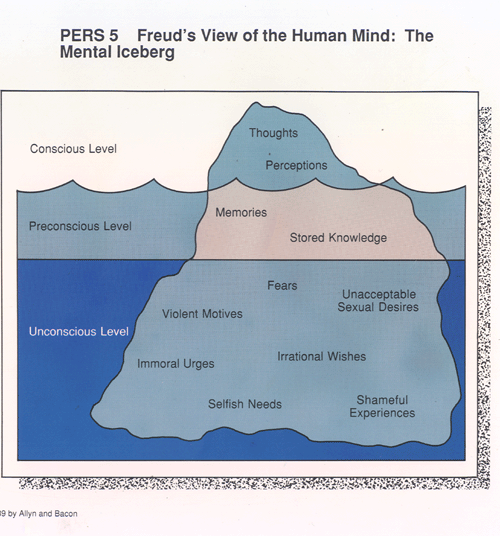
\includegraphics[width=0.5\linewidth]{modelloTopograficoDellaMente.png}
    \caption{Modello Topografico della mente}
    \label{Modello Topografico della mente}
\end{figure}

\clearpage

\end{document}